\documentclass{article}
\usepackage{booktabs}
\usepackage{amsmath}
\usepackage{graphicx}
\usepackage{caption}
\title{HW2}
\author{Zhijiia Chen}
\begin{document}
\maketitle

\paragraph{B.13} A program is running on a computer with a four-entry fully associa- tive (micro) translation lookaside buffer (TLB) (Figure B.33):

The following is a trace of virtual page numbers accessed by a program. For each access indicate whether it produces a TLB hit/miss and, if it accesses the page table, whether it produces a page hit or fault. Put an X under the page table column if it is not accessed (Figures B.34 and B.35).

\begin{table}[h!]
\begin{center}
    \caption{Page access trace}
    \label{tab:table1}
    \begin{tabular}{c|c|c} % <-- Alignments: 1st column left, 2nd middle and 3rd right, with vertical lines in between
    \toprule
    \textbf{Virtual page accessed} & \textbf{TLB (hit or miss)} & \textbf{Page table (hit or fault)}\\
    \hline
    1 & miss & fault\\
    \hline
    5 & hit & X\\
    \hline
    9 & miss & fault\\
    \hline
    14 & miss & fault\\
    \hline
    10 & hit & X\\
    \hline
    6 & miss & hit\\
    \hline
    15 & hit & X\\
    \hline
    12 & miss & hit\\
    \hline
    7 & miss & hit\\
    \hline
    2 & miss & fault\\
    \bottomrule
    \end{tabular}
\end{center}
\end{table}

\paragraph{2.18} You are investigating the possible benefits of a way-predicting L1 cache. Assume that a 64 KB four-way set associative single-banked L1 data cache is the cycle time limiter in a system. For an alternative cache organization, you are considering a way-predicted cache modeled as a 64 KB direct mapped cache with 80\% prediction accuracy. Unless stated otherwise, assume that a mispredicted way access that hits in the cache takes one more cycle. Assume the miss rates (0.030) and the miss penalties (20 cycles) in question 2.8 part (c).

\subparagraph{a.} What is the average memory access time of the current cache (in cycles) versus the way-predicted cache?

Suppose a cache hit time is 2 cycles for current cache. And for the way-predicated cashe, the hit time is 1 cycle if it prediction success and 3 cycles otherwise.

Average memroy access time for current cache: 2 + 0.030 $\times$ 20 = 2.6 cycles.

Average memroy access time for way-predicated cache: $0.97\times(0.8\times1+0.2\times3)+0.03\times(3+20)=2.048$ cycles.

\subparagraph{b.} If all other components could operate with the faster way-predicted cache cycle time (including the main memory), what would be the impact on performance from using the way-predicted cache?

$\frac{2.6}{2.048}=1.27$, so the performance could be 27\% faster.

\subparagraph{c.} Way-predicted caches have usually been used only for instruction caches that feed an instruction queue or buffer. Imagine that you want to try out way prediction on a data cache. Assume that you have 80\% prediction accuracy and that subsequent operations (e.g., data cache access of other instructions, dependent operations) are issued assuming a correct way prediction. Thus a way misprediction necessitates a pipe flush and replay trap, which requires 15 cycles. Is the change in average memory access time per load instruction with data cache way prediction positive or negative, and how much is it?

Average memroy access time for cache without way-predictor: 2.6 cycles.

Average memroy access time for way-predicated cache: $0.97\times(0.8\times1+0.2\times(3+15))+0.03\times(3+20)=4.958$ cycles.

So the change is negative, the average memroy access time would be increased by 2.358 cycles.

\begin{figure}[!htb]
\begin{center}
\begin{minipage}{.7\linewidth}
    \centering
    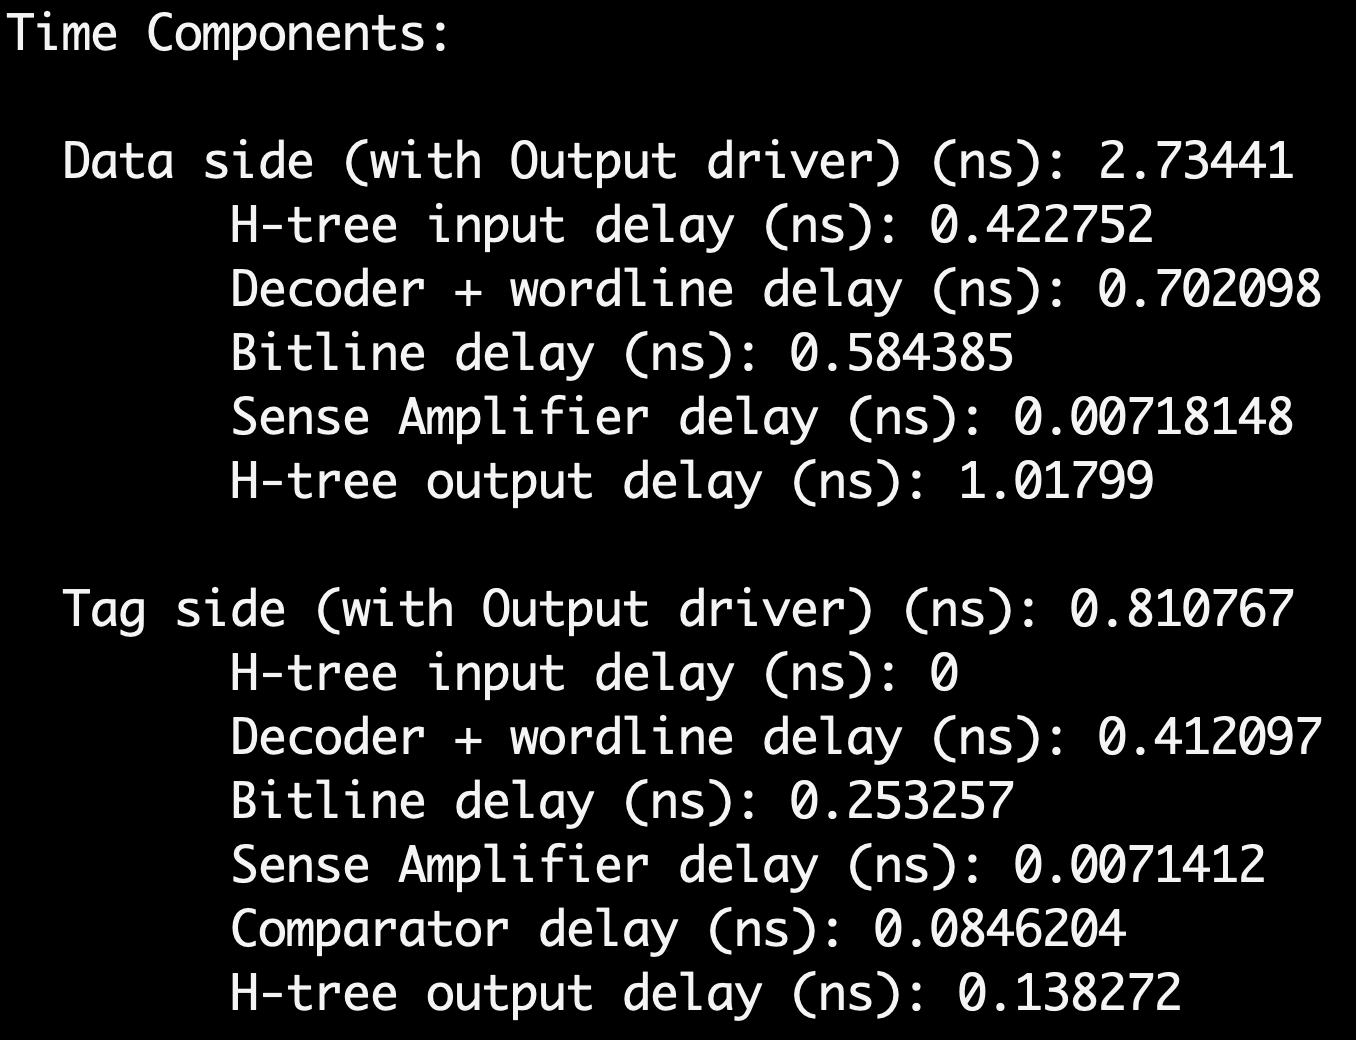
\includegraphics[width=1\linewidth]{./1.png}
    \captionof{figure}{\small CACTI time components results}
    \label{fig:CACTI} 
\end{minipage}
\end{center}
\end{figure}

\subparagraph{d.} As an alternative to way prediction, many large associative L2 caches serialize tag and data access so that only the required dataset array needs to be activated. This saves power but increases the access time. Use CACTI’s detailed web interface for a 0.065 m process 1 MB four-way set associative cache with 64-byte blocks, 144 bits read out, 1 bank, only 1 read/write port, 30 bit tags, and ITRS-HP technology with global wires. What is the ratio of the access times for serializing tag and data access compared to parallel access?

Figure~\ref{fig:CACTI} shows the time components of CACTI simulation results. The data side takes 2.734ns and the tag side takes 0.811ns. For parallel access, the access time is the dominant part between tag access time and data access time, while for serialized access, the access time is the time to access the tags plus the time to access the data, thus the ratio is: $\frac{0.811+2.734}{2.734}=1.297$.

\paragraph{2.20} Consider the usage of critical word first and early restart on L2 cache misses. Assume a 1 MB L2 cache with 64-byte blocks and a refill path that is 16 bytes wide. Assume that the L2 can be written with 16 bytes every 4 processor cycles, the time to receive the first 16 byte block from the memory controller is 120 cycles, each additional 16 byte block from main memory requires 16 cycles, and data can be bypassed directly into the read port of the L2 cache. Ignore any cycles to transfer the miss request to the L2 cache and the requested data to the L1 cache.

\subparagraph{a.} How many cycles would it take to service an L2 cache miss with and without critical word first and early restart?

Each block contains 4 words. For early restart, suppose each word has the same possibility to be the expected one.

Without critical word first and early restart, it requires 120 cycles for the first word, and 16 cycles for each of the following 3 words, thus $120+3\times16=168$ cycles.

With critical word first, it requires 120 cycles for the expected word.

With early restart, it requires 120 cycles for the first word, and the expected cycles to wait for the remaining ones. So the expected cycles = $120 + 0.25\times(0 + 16 + 32 + 48) = 148$ cycles.

\subparagraph{b.} Do you think critical word first and early restart would be more important for L1 caches or L2 caches, and what factors would contribute to their relative importance?

I think critical word first and early restart are more important for L2 caches, because L2 caches has larger cache block size, and we don't have to wait the whole large block. For the L1 cache where the block is generally smaller, the improvement may not worth the overhead.

\paragraph{2.21} You are designing a write buffer between a write-through L1 cache and a write-back L2 cache. The L2 cache write data bus is 16 B wide and can perform a write to an independent cache address every four processor cycles.

\subparagraph{a.} How many bytes wide should each write buffer entry be?

The write buffer entry should match the write data bus, i.e., 16 B.

\subparagraph{b.} What speedup could be expected in the steady state by using a merging write buffer instead of a non-merging buffer when zeroing memory by the execution of 64-bit stores if all other instructions could be issued in parallel with the stores and the blocks are present in the L2 cache?

Each store writes 8 B. Suppose each entry of the write buffer is 16 B.

With merging write buffer, each write cycle can write 16 B, while with non-merging write buffer, each write can only write 8 B. So the merging write buffer is 100 \% faster.

\subparagraph{c.} What would the effect of possible L1 misses be on the number of required write buffer entries for systems with blocking and non-blocking caches?

If L1 is a blocking cache, then the processor has to wait until the missed block has been loaded into the cache, so the misses do not affects the required number of write buffers entries in L2 cache. While if L1 is a non-blocking cache, the processor can still write to the write buffer during misses, thus fewer write buffer entries may be required.

\paragraph{2.33} Consider a desktop system with a processor connected to a 2 GB DRAM with error-correcting code (ECC). Assume that there is only one memory channel of width 72 bits (64 bits for data and 8 bits for ECC).

\subparagraph{a.} How many DRAM chips are on the DIMM if 1 Gb DRAM chips are used, and how many data I/Os must each DRAM have if only one DRAM connects to each DIMM data pin?

With 8 bits ECC for 64 bits data, it means there is one bit overhead for every byte transmitted. 2 GB = 16 Gb, and with another 2 Gb overhead, there should be 18 1 Gb DRAM chips on the DIMM.

To achieve 72 bits output bandwidth, $\frac{72}{18}=4$ I/Os are needed.

\subparagraph{b.} What burst length is required to support 32 B L2 cache blocks?

The effective channel width is 64 bits = 8 B, so a burst length of 4 is required.

\subparagraph{c.} Calculate the peak bandwidth for DDR2-667 and DDR2-533 DIMMs for reads from an active page excluding the ECC overhead.

Peak bandwidth for DDR2-667 = 8$\times$667 = 5336 MB/s.

Peak bandwidth for DDR2-533 = 8$\times$533 = 4264 MB/s.

\paragraph{2.37} Consider a processor that has four memory channels. Should consecutive memory blocks be placed in the same bank, or should they be placed in different banks on different channels?

If the consecutive blocks can be fitted within one row, then they should be placed in the same bank, otherwise they should be placed in different banks with each bank holding part of the consecutive blocks in one row, so closing the row and precharging can overlap with accessing the new row.

\paragraph{2.41} Virtual machines (VMs) have the potential for adding many beneficial capabilities to computer systems, such as improved total cost of ownership (TCO) or availability. Could VMs be used to provide the following capabilities? If so, how could they facilitate this?

\subparagraph{a.} Test applications in production environments using development machines?

Yes, the development machines can make a VM with production specified environments for the applications.

\subparagraph{b.} Quick redeployment of applications in case of disaster or failure?

Yes, when disaster or failure happens to the physical machines, the VM can be quickly exported to backup machines.

\subparagraph{c.} Higher performance in I/O-intensive applications?

No, VM has significantly decreased performance in I/O related takes, so it is not suitable for I/O-intensive applications.

\subparagraph{d.} Fault isolation between different applications, resulting in higher availability for services?

Yes, Suppose each application are running inside its own VM, then they are isolated with each other and the crashing of one VM would not affect other VMs.

\subparagraph{e.} Performing software maintenance on systems while applications are running without significant interruption?

No. The VM are running on the host. The VM cannot get regular performance when the underlying host system is undergoing maintenance.

\end{document}